\documentclass[11pt,a4paper]{article}

\usepackage[margin=1in]{geometry}
\usepackage{amsmath}
\usepackage{hyperref}
\usepackage{tikz}
\usepackage{float}
\usepackage{parskip}
\usepackage{adjustbox}

\usetikzlibrary{positioning, arrows.meta}

\title{Covering Singapore's Bus Network via Directed Graph Traversal}
\author{Ryan Pek}
\date{\today}

\begin{document}

\maketitle

\section{Problem Statement}

Given a directed graph $G=(V,E)$ representing bus stops and valid bus-route
transitions, construct a walk starting from a chosen vertex $s$ that visits
every vertex $v \in V$ at least once.

An ideal case is to visit each vertex exactly once, which corresponds to finding
a Hamiltonian Cycle or Hamiltonian Path.

However, because the network is directed and constrained by actual bus routes, 
my intuition is that repeated visits may be necessary to visit all the stops.

After construction of the graph, the objectives of follow up algorithms are
to minimise the number of repeated vertices, such that the final walk returns
a solution that approximates that of a Hamiltonian cycle.

\section{Project Approach}

A summary of what the project consists of:
\begin{itemize}
    \item A data ingestion pipeline that fetches and stores raw LTA data
    \item A preprocessing step that constructs a compact graph representation
    \item A set of algorithms operating on the in-memory graph to compute covering walks
\end{itemize}

\section{Data Gathering}

The graph is built from LTA bus data. Raw JSON snapshots are stored first, then
processed into a compact adjacency-list representation.

\begin{figure}[H]
\centering
\begin{adjustbox}{max width=\textwidth}
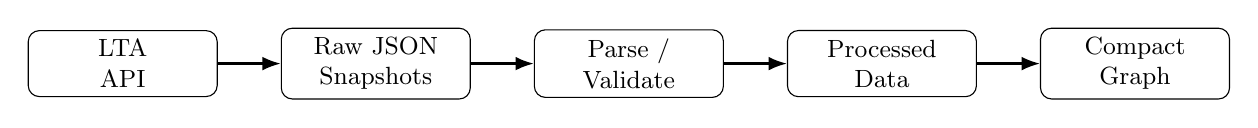
\begin{tikzpicture}[
    node distance=0.8cm,
    box/.style={
        draw,
        rounded corners,
        align=center,
        minimum width=2.4cm,
        minimum height=0.8cm,
        font=\small
    },
    arrow/.style={-Latex, thick}
]

\node[box] (api) {LTA\\API};
\node[box, right=of api] (raw) {Raw JSON\\Snapshots};
\node[box, right=of raw] (parse) {Parse /\\Validate};
\node[box, right=of parse] (processed) {Processed\\Data};
\node[box, right=of processed] (graph) {Compact\\Graph};

\draw[arrow] (api) -- (raw);
\draw[arrow] (raw) -- (parse);
\draw[arrow] (parse) -- (processed);
\draw[arrow] (processed) -- (graph);

\end{tikzpicture}
\end{adjustbox}
\caption{Data gathering and preprocessing pipeline.}
\end{figure}

\section{Graph Model}

Each bus stop is represented as a vertex. A directed edge $(u,v)$ exists if a
bus can travel directly from stop $u$ to stop $v$ along a valid service route.

\begin{figure}[h]
\centering
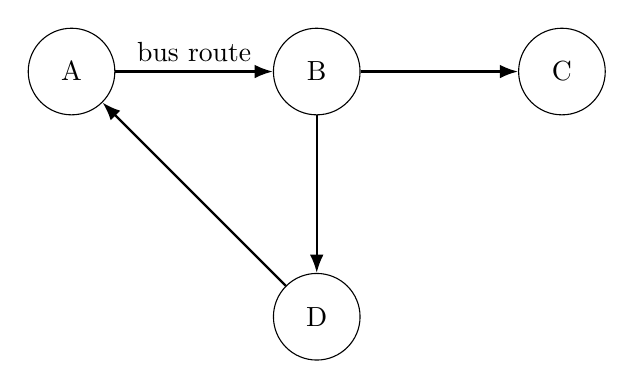
\begin{tikzpicture}[
    node distance=2cm,
    stop/.style={
        circle,
        draw,
        minimum size=1.1cm
    },
    arrow/.style={-Latex, thick}
]

\node[stop] (a) {A};
\node[stop, right=of a] (b) {B};
\node[stop, right=of b] (c) {C};
\node[stop, below=of b] (d) {D};

\draw[arrow] (a) -- node[above] {bus route} (b);
\draw[arrow] (b) -- (c);
\draw[arrow] (b) -- (d);
\draw[arrow] (d) -- (a);

\end{tikzpicture}
\caption{Directed graph model of bus-stop transitions.}
\end{figure}

\section{Objectives}

\begin{itemize}
    \item Visit every bus stop at least once
    \item Minimise repeated visits
    \item Minimise total distance
    \item Return to the starting vertex if possible
\end{itemize}

\section{Follow Up}

Follow up papers will describe:

\begin{itemize}
    \item Graph construction and validation
    \item Heuristic and algorithmic approaches for vertex-covering walks
    \item Analysis of structural properties (betweenness, flow, chokepoints)
\end{itemize}

\section{Project History}

The initial version of this project was implemented in Python as an exploratory
prototype to understand the structure of the bus network and to experiment with
basic traversal strategies.

The system consisted of multiple components:

\begin{itemize}
    \item A set of scripts to query the LTA DataMall APIs and store responses as JSON files
    \item Processing functions that extracted relevant information such as bus services,
    routes, and stop metadata
    \item A large number of intermediate JSON files, including per-stop data and per-route data
    \item A traversal module (Traveller) that attempted to explore the graph and visit all stops
\end{itemize}

While functional, this design had several limitations:

\begin{itemize}
    \item Heavy reliance on file-based JSON storage, resulting in thousands of small files
    \item Repeated parsing and scanning of JSON data during execution
    \item Tight coupling between data access, processing, and traversal logic
    \item Inefficient lookup patterns, often requiring linear scans over multiple files
    \item Difficulty reasoning about performance due to mixed concerns
\end{itemize}

In particular, many queries such as retrieving the direction, distance, or adjacency
of a bus stop required iterating through multiple JSON datasets repeatedly. This
introduced significant overhead and made the system difficult to scale.

These limitations motivated a redesign of the system, focusing on:

\begin{itemize}
    \item Separating data ingestion, preprocessing, and algorithmic components
    \item Constructing a single compact in-memory graph representation
    \item Reducing repeated file I/O and JSON parsing
    \item Improving performance and clarity of the traversal algorithms
\end{itemize}

The current work represents the beginning of this redesign, with a transition to Go
and a focus on building a more efficient and modular system.

\end{document}
